\documentclass{article}
\usepackage{tikz}
\usepackage{todonotes}
\usepackage{amssymb}
\usepackage{amsmath}
\usetikzlibrary{arrows,decorations.pathmorphing,shapes.multipart}

\hyphenation{Schwell-werte}
% =============== Definitionen =========
\newenvironment{definition}
    [1]
    {
        {\bf Definition:} #1\\
    }
    {}

\newcommand{\defined}
    [1]
    {
        {\bf #1}
    }
% ======================================

% =============== Requirements =========
\newcounter{requirementscount}{}
\setcounter{requirementscount}{0}
\newcommand{\requirement}[1] {
        \addtocounter{requirementscount}{1}
        {\bf Requirement \therequirementscount:} #1\\
    }

% =============== PHASES ===============
\newcounter{ycounter}{}
\newenvironment{phases}
{
\setcounter{ycounter}{-1}
\begin{tikzpicture}[node distance=3cm,text width=3cm,
    box/.style={shape=rectangle,draw}]
}
{\end{tikzpicture}}

\newcommand{\nomoreheaders} {
    \addtocounter{ycounter}{-1}
}

\newcommand{\aliceheader}[1] {
\node at (-4,\theycounter) {#1}
}
\newcommand{\bobheader}[1] {
\node at (4,\theycounter) {#1}
}

\newcommand{\aliceknowledge}[2][0]{
\node[box]
    at (-4+#1, \theycounter)
    {#2}
}
\newcommand{\bobknowledge}[2][0]{
\node[box]
    at (4+#1, \theycounter)
    {#2}
}

\newcommand{\symmetricknowledge}[2][0]{
\aliceknowledge{#2};
\bobknowledge[#1]{#2};
}


\newcommand{\phase}[1]{
\addtocounter{ycounter}{-1};
\draw[->,decorate,decoration={snake,amplitude=1mm,post length=2mm}]
    (0,\theycounter) -- ++(0,-2)
    node [right,midway,xshift=3mm] {#1};
\addtocounter{ycounter}{-3};
}
% ======================================

\begin{document}
\listoftodos
\pagebreak
\tableofcontents
\pagebreak
\section{Einleitung}
\todo[inline]{Struktur vom Dokument erl\"autern}
\subsection{Begriffe}
\begin{definition}{Eigenes,Gesamtes}
\(M\) sei eine Menge von Elementen, die in zwei Teilmengen \(M_A\)
und \(M_B\) zerf\"allt, sodass \(M = M_A \cup M_B\) ist. Wir nehmen
desweiteren an, dass Alice \(M_A\) kennt, aber weder \(M\) noch \(M_B\)
und dass foo Bob \(M_B\) kennt, aber weder \(M\) noch \(M_A\). Dann bezeichnen
wir:
\begin{itemize}
\item \(M\) als \defined{gesamtes} Wissen
\item \(M_A\) als das \defined{eigene} Wissen von Alice
\item \(M_B\) als das \defined{eigene} Wissen von Bob
\item \(M_B\) als das \defined{andere} Wissen von Alice
\item \(M_A\) als das \defined{andere} Wissen von Bob
\end{itemize}
\end{definition}
\begin{definition}{Gemeinsam}
Wenn beide Anwender das gleiche Wissen w haben, dann bezeichnen wir w
als \defined{gemeinsames Wissen}. 
\end{definition}\\
\begin{definition}{Vorwissen}
Wenn Anwender verschiedene Phasen hintereinander ausf\"uhren, dann bezeichnen
wir das Wissen aus den bereits ausgef\"uhrten Phasen als \defined{Vorwissen}.
\end{definition}\\
\todo[inline]{Definition: Entscheidungsbaum}
\begin{definition}{Attribut}
Wir definieren eine Menge von Wahrscheinlichkeiten 
\(P = [0, 1] \subset \mathbb{R}\) und eine Menge von Buchstaben 
\(\Sigma = \{a, b, \dots, z, A, B, \dots, Z\}\).
Damit definieren wir ein \defined{Attribut} als 
\(\Sigma^+ \times P \times P\). Wenn ein Attribut \(A = (w, l, h)\) gegeben ist,
bezeichnen wir w als \defined{Wort}, l als \defined{unterer Schwellwert} und h
als \defined{oberer Schwellwert}. Es wird desweiteren von allen Attributen
gefordert, dass \(l \leq h\) ist.
\end{definition}\\
\begin{definition}{Wahrheitstafel}
F\"ur eine boolsche Funktion ist eine \defined{Wahrheitstafel} eine Tabelle,
die f\"ur jede Kombination der Eingaben genau eine Ausgabe der beschriebenen
Funktion definiert.
\end{definition}\\
\begin{definition}{entstellte Wahrheitstafel}
Gegeben sei eine Wahrheitstafel mit Eingabevariablen 
\(\{i_1, i_2, \dots, i_n\}\) und Ausgabevariable o und wir 
 stellen f\"ur jede Variable v eine bijektive
 Verschleierung \(f_v : {0, 1} \mapsto \mathbb{Z}\) auf. 
Dann entsteht eine entstellte Wahrheitstafel f\"ur W, wenn
 wir f\"ur jede Zeile in der Wahrheitstafel die verschleierte Ausgabe
 mittels einer symmetrischen Verschl\"usselung mit den 
 verschleierten Werte der Eingangsvariablen in einem 
 Verschl\"usselungsschritt pro Eingangsvariable verschl\"usseln.
Es ist notwendig zu bemerken, dass eine Implementierung
 einen Weg anbieten muss, eine sinnlose Verschl\"usselung
 zu erkennen.\\
Wenn also beispielsweise in einer Wahrheitstafel die Eingaben 
 1 und 1 auf 1 abgebildet werden und die erste Eingabevariable
 verschleiert 1 als 23, die zweite Eingabevariable verschleiert
 1 als 49 und die Ausgabevariable verschleiert 1 als 12 und E
 ist die symmetrische Verschlueselung, dann
 ist das daraus entstehende Element der entstellten Wahrheitstafel
 \(E_{f_{i_1}(1)}(E_{f_{i_2}(1)}(f_o(1))) = E_{49}(E_{23}(12))\)
\end{definition}\\
\begin{definition}{Schaltkreis}
Wir definieren einen \defined{Schaltkreis} als einen gerichteten azyklischen 
 Graphen.
Die Knoten dieses Graphen sind annotiert mit Wahrheitstafeln. 
Die Kanten sind eingeteilt in \defined{Eingabekanten}, \defined{innere Kanten} 
 und \defined{Ausgangskanten}.
Der Wert einer Eingabekante wird vom Anwender zu Beginn festgelegt. 
Der Wert einer inneren Kante oder einer Ausgangskante ergibt sich durch
 anwenden der Wahrheitstafel auf die Eingangskanten. 
Da wir nur boolsche Schaltkreise mit den Knotenannotationen ,,and'',
 ,,or'', ,,xor'' und ,,not'' brauchen und all diese Funktionen entweder
 un\"ar oder kommutativ sind, brauchen wir keine Ordnung der Eingabekanten
 festlegen.
\end{definition}\\
\begin{definition}{Entstellter Schaltkreis}
Ein \defined{entstellter Schaltkreis} entsteht aus einem normalen Schaltkreis,
 indem jede an einen Knoten annotierte Wahrheitstafel entstellt wird, wenn
 dabei garantiert wird, dass f\"ur die Verbindung einer Ausgangsvariablen
 o mit einer Eingangsvariablen i auf beide Variablen die gleiche
 Verschleierung angewendet wird.\\
Desweiteren wird f\"ur jede Eingabekante die Verschleierungsfunktion
 gespeichert, um die Eingabe des Schaltkreises kodieren zu k\"onnen und
 f\"ur jede Ausgangskante die Inversion der Verschleierungsfunktion
 gespeichert, um die Ausgabe dekodieren zu k\"onnen.
\end{definition}
\subsection{Annahmen}
\todo[inline]{Annahme: ehrliche anwender := "handeln nach protokoll"}

\pagebreak
\section{Grundlagen der Anwendung}
\todo[inline]{Vision der Anwendung}

\subsection{Form der Benutzereingabe}
\todo[inline]{Festlegen, wie die E-Mails ins Programm kommen}

\subsection{Interaktion der verteilten Programme}
\todo[inline]{Festlegen, wie das Programm verteilt wird und die Teile kommunizieren}
\todo[inline]{Austauschen der Anzahl der E-Mails}

\subsection{Phasen der Anwendung}
\todo[inline]{Kurz die Einzelnen phasen der Anwendung beschreiben}
\begin{figure}[htb]
\centering
\begin{phases}
\aliceheader{Alice};
\bobheader{Bob};
\nomoreheaders
\aliceknowledge[-2]{eigene E-Mails};
\bobknowledge[-2]{eigene E-Mails};

\aliceknowledge[2]{Einordnung von eigenen E-Mails als Spam, Nicht Spam};
\bobknowledge[2]{Einordnung von eigenen E-Mails als Spam, Nicht Spam};

\phase{Phase 1: Finden der gemeinsamen Wortliste};

\symmetricknowledge{Gemeinsame Wortliste};

\phase{Phase 2: Finden der gemeinsamen Schwellwerte};

\symmetricknowledge{Gemeinsame Attribute = Liste von (Wort + Schwellwerte)};
\phase{Phase 3: Diskretisieren der eigenene E-Mails};

\symmetricknowledge{Eigene diskretisierte E-Mails};

\phase{Phase 4: Lernen der gesamten E-Mails};

\symmetricknowledge{Gemeinsamer Klassifikator};
\end{phases}
\caption{Phasen der Anwendung}
\end{figure}


\pagebreak % XXX: if possible, kill this pagebreak
\section{Finden der gemeinsamen Wortliste}
In dieser Phase berechnen die beiden Parteien aus den gesamten E-Mails
eine gemeinsame Wortliste, die mit grosser Wahrscheinlichkeit 
aussagekr\"aftige Attribute f\"ur den Entscheidungsbaum liefert. 
Die Phase besteht aus zwei Schritten.
Im ersten Schritt berechnen beide Parteien getrennt eine eigene Wortliste.
Jedes Wort auf dieser Liste hat in den eigenen E-Mails hat eine starke 
 Aussagekraft \"uber die Klassifikation der E-Mails, die das Wort
 oft enthalten.
Im zweiten Schritt vereinen beide Parteien ihre eigenen Wortlisten, um 
 die gemeinsame Wortliste zu berechnen. 
Dieser Vorgang ist in Abbildung ~\ref{fig:phase:two} illustriert.

\begin{figure}[h!tb]
\begin{phases}
\aliceheader{Alice};
\bobheader{Bob};
\nomoreheaders

\aliceknowledge[-2]{eigene E-Mails};
\bobknowledge[-2]{eigene E-Mails};

\aliceknowledge[2]{Einordnung von eigenen E-Mails als Spam, Nicht Spam};
\bobknowledge[2]{Einordnung von eigenen E-Mails als Spam, Nicht Spam};
\phase{Phase 1.1.1: Berechnung der Anteile der Worte in eigenen Spam/Nicht Spam E-Mails};
\symmetricknowledge[1]{Liste von (Wort + Anteil der Vorkomnisse eines Wortes an allen eigenen Worten)};
\phase{Phase 1.1.2: Auswahl der N besten eigenen Worten nach Informationsheuristik};
\symmetricknowledge{Eigene Wortliste}
\phase{Phase 1.2: Synchronisierung der Wortlisten}
\symmetricknowledge{Gemeinsame Wortliste}
\end{phases}
\caption{Schritte zum Berechnen der gemeinsamen Wortliste}
\label{fig:phase:two}
\end{figure}

\subsection{Berechnung der Anteile an den Wortmengen}
Wir verwenden eine Heuristik f\"ur den Informationsgehalt des Vorkommens eines
Wortes in einer E-Mail, die auf dem Verh\"altnis der Vorkommnisse des 
Wortes zu der Gesamtanzahl Worte in einer Klasse basiert. 
Um diese zu berechnen werden konzeptionell alle Worte in E-Mails einer Klasse 
 zu einer Multimenge hinzugef\"ugt. 
F\"ur jedes Wort in dieser Multimenge ist das Verh\"altnis der
Vielfachheit des Wortes zur M\"achtigkeit der Multimenge das gesuchte
Verh\"altnis.
Damit ergibt sich folgendes Akzeptanzkriterium:\\
\requirement{Wenn die Spam-Mails die Mails "Foo Bar", "Foo Bar", "Foo Foo"
und "Foo" sind und die Nicht-Spam-Mails "Bar Bar", "Foo" und "Bar", 
dann muss diese Phase die folgende Tabelle berechnen:\\
\begin{center}
\begin{tabular}{c c c}
Wort & Spam-Anteil & Nicht-Spam-Anteil \\
Foo & \(\frac{5}{7}\) & \(\frac{1}{4}\) \\
Bar & \(\frac{2}{7}\) & \(\frac{3}{4}\)
\end{tabular}
\end{center}
Eine Approximation der Werte durch Fliesskommazahlen ist
ebenfalls akzeptabel.}

\subsection{Auswahl der Worte nach Informationsheuristik}
Wir wollen nun Worte ausw\"ahlen, deren h\"aufiges Vorkommen in einer
 E-Mail viel \"uber die Klasse der E-Mail aussagen.
Wir verwenden dabei eine deduktive Heuristik, die annimmt, dass die
 Wahrscheinlichkeit, dass eine E-Mail zu einer Klasse geh\"ort, direkt
 mit den Wahrscheinlichkeiten zusammenh\"angt, dass die W\"orter in
 dieser E-Mail zu dieser Klasse geh\"oren. 
Das bedeutet, wir wollen Worte selektieren, bei denen genau eine 
 Wahrscheinlichkeit, zu einer Klasse zu geh\"oren, drastisch unterschiedlich
 ist.\\
Eine m\"ogliche Quantifizierung dieser Unterschiedlichkeit ist im bin\"aren
 Fall \(\Delta(x, y) = \|x - y\|\).
Diese Quantifizierung hat die Eigenschaft, f\"ur 
 x = 1 und y = 0 bzw x = 0 und y = 1 maximal 1 zu sein, und f\"ur identische 
 x und y 0 zu sein. 
Da x und y f\"ur die Belegung (0, 1) bzw (1, 0) wirklich maximal weit 
 auseinander liegen und bei gleichen Werten wirklich die gerinstm\"ogliche
 Aussage \"uber die Klassezugeh\"origkeit eines Wortes getroffen wird, 
 ist dies wirklich eine Quantifizierung der Aussagekraft, die wir anstreben. 
Damit w\"ahlen wir die aussagekr\"aftigstenen Worte aus, indem wir alle Worte 
    nach 
\(\Delta(\mathrm{Vorkommen~in~Spam-E-Mails}, 
         \mathrm{Vorkommen~in~Nicht-Spam-E-Mails})\) 
 absteigend sortieren und die ersten N Worte w\"ahlen. 
Damit ergibt sich folgendes Akzeptanzkriterium:\\
\requirement{Wenn N = 2 ist, und als Worte mit Vorkomnissen gegeben sind:
\begin{center}
\begin{tabular}{c c c}
Wort & Vorkomnisse in Spam-E-Mails & Vorkommnisse in Nicht-Spam-Emails \\
A & 0.5 & 0.5 \\
B & 0.2 & 0.2 \\
C & 0.3 & 0.5 \\
D & 0.2 & 0.8 \\
E & 0.9 & 0.2
\end{tabular}
\end{center}
dann werden als Wortliste D und E gew\"ahlt.}

\subsection{Zusammenfassen der Wortlisten}
Wir haben nun zwei separate, lokale Wortlisten berechnet. Diese m\"ussen
zusammengefasst werden zu einer gemeinsamen Wortliste. Da wir annehmen, dass
die Benutzer ehrlich sind, k\"onnen wir annehmen, dass die Benutzer als
Eingabe dieses Protokolles keine beliebige Liste festlegen und auch ihre
Daten nicht so manipulieren, dass eine bestimmte Wortliste versendet wird.
Zudem werden die Attribute des Baumes \"offentlich sein, sodass eine
Geheimhaltung der Wortlisten keinen Sinn macht.
Deswegen k\"onnen wir die Wortlisten durch eine einfache Vereinigung der
separaten Wortlisten zu einer gesamten Wortliste vereinigen. Deswegen wird 
das Zusammenfassen der Wortliste implementiert, indem beide Anwender ihre
lokale Wortliste an den jeweils anderen Anwender versenden und beide 
Anwender lokal die Wortlisten vereinigen. Damit ergibt sich folgendes
Akzeptanzkriterium:\\
\requirement{Wenn Alice die Wortliste A, B, C berechnet hat, und Bob die
Wortliste C, D, E berechnet hat, dann muss die zusammengefasste Wortliste
A, B, C, D, E sein.} 

\pagebreak % XXX: if possible, kill this pagebreak
\section{Finden der gemeinsamen Schwellwerte}
\todo[inline]{Einleitung, auf Figure f\"ur Schwellwerte verweisen}

\begin{figure}[htb]
\begin{phases}
\aliceheader{Alice};
\bobheader{Bob};
\nomoreheaders

\aliceknowledge[-2]{Vorwissen};
\aliceknowledge[2]{Gemeinsame Wortliste};

\bobknowledge[-2]{Vorwissen};
\bobknowledge[2]{Gemeinsame Wortliste};
\phase{Phase 2.1: Berechnung der Vorkommnisse der Worte in eigenen Spam/Nicht Spam E-Mails};
\symmetricknowledge[1]{Eigene Liste von (Wort + Anteil der Vorkomnisse eines Wortes an Spam/Nicht-Spam Worten)};
\phase{Phase 2.2: Bestimmung eines Schwellwertes, der Spam, Nicht-Spam Anteile m\"oglichst halbiert};
\symmetricknowledge{Eigene Liste von (Wort + Schwellwert)};
\phase{Phase 2.3: Synchronisierung der Schwellwerte};
\symmetricknowledge{Gemeinsame Liste von (Wort + Schwellwerte)};
\end{phases}
\end{figure}
\todo[inline]{F\"ur section-Titel besseren Begriff f\"ur "Vorkomnisse der Worte in eigenen Spam/Nicht Spam E-Mails" finden}
\subsection{Berechnung der Anteile}
\todo[inline]{Content: Mittlwerte ausrechnen}
\subsection{Bestimmung der eigenen Schwellwerte}
Es muss nun f\"ur ein Wort \(w\) eine Schwelle gefunden werden, ab wann das
Wort w in einer E-Mail oft vorkommt. Wir w\"ahlen hierzu den Mittelwert
der Vorkomnisse des Wortes in allen eigene E-Mails eines Anwenders, da wir
dann die Begriffe ,,\"uberdurchschnittlich oft'' bzw ,,unterdurchschnittlich 
oft''als eigenen Schwellwert quantifizieren.
Damit ergibt sich folgendes Akzeptanzkriterium:\\
\requirement{Wenn die E-Mails "A A A", "A B B", "A C C" und "A A C" sind, dann
muss die Software als eigenen Mittelwert f\"ur das Wort A 
\(\frac{1}{4} \cdot (1 + \frac{1}{3} + \frac{1}{3} + \frac{2}{3}) = \frac{7}{12}\) bestimmen.}
\subsection{Syncronisierung der Schwellwerte}
\todo[inline]{Content: Alice a, Bob b -> <a, b>, unter dem minimum der beiden werte def. selten,
ueber dem max der werte def. oft und dazischen keine ahnugn. Implementierung als simples herumschicken}

\pagebreak % XXX: if possible, kill this pagebreak
\section{Diskretisieren der eigenen E-Mails}
\todo[inline]{Einleitung, Figure referenzieren}
\todo[inline]{Content}
\begin{figure}[htb]
\begin{phases}
\aliceheader{Alice};
\bobheader{Bob};
\nomoreheaders;
\aliceknowledge[-2]{Vorwissen};
\aliceknowledge[2]{Gemeinsame Attribute = Liste von (Wort + Schwellwerte)};

\bobknowledge[-2]{Vorwissen};
\bobknowledge[2]{Gemeinsame Attribute = Liste von (Wort + Schwellwerte)};

\phase{Phase 3: Diskretisieren der eigenene E-Mails};
\symmetricknowledge{Eigene diskretisierte E-Mails};
\end{phases}
\end{figure}

\pagebreak % XXX: if possible, kill this pagebreak
\section{Lernen der gesamten E-Mails}
\todo[inline]{verteiltes ID3 beschreiben}

\subsection{Yaos Protokoll}
\begin{figure}[htb]
\begin{phases}
\aliceheader{Alice};
\bobheader{Bob};
\nomoreheaders
\aliceknowledge[-2]{Eigene Eingabe};
\aliceknowledge[2]{Schaltkreis};

\bobknowledge[-2]{Eigene Eingabe};
\bobknowledge[2]{Schaltkreis};

\phase{Y.1: Konstruktion des entstellten Schaltkreises und \"Ubertragung};
\aliceknowledge[-2]{Eingabekodierung};
\aliceknowledge[2]{entstellter Schaltkreis};
\bobknowledge{entstellter Schaltkreis};
\phase{Y.3 Alice schickt kodierte Eingabe an Bob};
\bobknowledge{Alice' kodierte Eingabe};
\phase{Y.4 Via Oblivious Transfer wird Bob's Eingabe kodiert};
\bobknowledge{Bob's kodierte Eingabe};
\phase{Y.5 Bob wertet Schaltkreis aus und sendet die Ausgabe an Alice};
\symmetricknowledge{Ausgabe} ;
\end{phases}
\caption{Yaos Protokoll}
\end{figure}
Die Eingabe jedes Anwenders f\"ur Yaos Protokoll ist eine Eingabe, und nach
Kerckhoffs Prinzip auch der auszuf\"uhrende Schaltkreis in Reinform. Einer
der beiden Anwender, ohne Beeintraechtigung der Allgemeinheit Alice, muss
nun aus diesem Schaltkreis einen enstellten Schaltkreis konstruieren. Dies
kann am einfachsten passieren, indem der Schaltkreis in einer Breitensuche
traversiert wird und die Kanten verschleiert werden. Das bedeutet, dass
in einem Schritt die zusammenh\"angenden Eingangs- und Ausgangsvariablen 
verschleiert werden. Dadurch werden die Anforderungen aus der Definition
der entstellten Schaltkreise erf\"ullt. Dabei kann dann auch erkannt
werden, dass eine Eingangsvariable bzw Ausgabevariable kein ,,anderes
Ende'' hat, d.h. diese Verschleierung in die Eingabekodierung bzw
Ausgabekodierung geschrieben werden muss. Dieser Schaltkreis und die
Ausgangskodierung wird dann an Bob \"ubertragen, w\"ahrend die
Eingangskodierung bei Alice verbleibt.\\
Bei der Verschl\"usselung der Ausgaben verwenden wir ein einfaches XOR.
Um zu garantieren, dass wir Unsinnige Verschl\"usselungen erkennen k\"onnen,
erweitern wir jeden Tabelleneintrag um eine zweiten Tabelleneintrag, der 
aus einem analog zum Nutzeintrag verschl\"usselten Nullvektor besteht.
Wir bezeichnen diesen Eintrag als
Markierungseintrag. Dann ist es m\"oglich, diesen Eintrag
zu entschl\"usseln, zu \"uberpr\"ufen, ob dies der 0-Vektor ist und falls dies
der Fall ist, den Nutzeintrag zu entschl\"usseln. Der einzige Fall, wo dies
Probleme bereitet ist, wenn die bei zwei Eingaben die Verschleierungen 
genau kontr\"ar sind, da dann \(a \oplus b = 0 = b \oplus a\) gilt
und somit die Eingabe (0,1) und (1,0) die gleiche Ausgabe liefert. Dies
muss also beim Verschleiern verhindert werden, was jedoch kein Problem ist.\\
Bob muss nun noch die Belegung der Eingangskanten lernen. Die
Eingabevariablen, die von Alice Eingabe belegt werden m\"ussen werden
belegt, indem Alice anhand der Eingangskodierung ihre Eingabe kodiert
und diesen String an Bob versendet. Da Bob keine Informationen dar\"uber
hat, welcher der beiden Verschleierungswerte f\"ur 0 oder f\"ur 1 steht,
erh\"alt Bob damit keine Informationen \"uber Alice Eingabe.\\
F\"ur die Kodierung von Bob's Eingabe muss etwas mehr Aufwand getrieben
werden, da weder Bob die Eingabekodierung lernen darf (weil er sonst
Alice Eingabe lernt), noch Alice Bob's Eingabe lernen darf (indem z.B.
Bob seine Eingabe an Alice schickt, damit Alice die Eingabe kodieren kann).
Daher wird dies durch eine Anwendung des 1-2-Oblivious-Transfers gel\"ost:
Alice bietet f\"ur jede von Bob zu belegende Eingabevariable die Werte
f\"ur 0 bzw 1 an, und Bob w\"ahlt mithilfe seines Eingabebits den richtigen
Wert aus. Aus den Eigenschaften von OT folgt, dass Alice nicht weiss, welchen
der beiden Werte Bob gew\"ahlt hat, und dass Bob den nicht gew\"ahlten Wert
nicht kennt. Somit ist die Sicherheit von Bobs Eingabe gegeben und 
sichergestellt, dass Bob wirklich seine Eingabe verwendet.\\
Wir implementieren den 1-2 Oblivious Transfer mittels RSA. Die Eingabe
von Alice seien \(m_1\), \(m_2\) und die Eingabe von Bob sei \(b\).
Alice ein Schl\"usselpaar, den privaten Exponenten e, den
\"offentlichen Exponenten d und sendet den Modulus N, d und zwei zuf\"allige
Nachrichten \(x_1\) und \(x_2\) an Bob. Bob w\"ahlt eine zuf\"allige Nachricht
k, verschl\"usselt k zu \(k'\) und sendet \(v = x_b + k' mod N\) an Alice. 
Alice berechnet nun \(k_0\) als Entschl\"usselung von \(v - x_0\) und 
\(k_1\) als Entschl\"usselung von \(v - x_1\) und sendet \(m_0 + k_0\) und
\(m_1 + k_1\) an Bob. Wenn Bob b = 0 gew\"ahlt hatte, kann Bob \(m_0\)
durch Subtraktion von \(k'\) von Alice erster Nachricht berechnen, und wenn
Bob b = 1 gew\"ahlt hatte, kann Bob \(m_1\) durch Subtraktion von \(k'\) von
Alice zweiter Nachricht berechnen. Das folgt (oBdA f\"ur b = 0) aus
\(m_0 + k_0 - k' = m_0 + D(v - x_0) - k' = m_0 + k' - k' = m_0\). Falls b 
nicht 0 war, heben sich in der Entschl\"usselung die Faktoren \(x_0\) und
\(x_1\) nicht auf und ein undefinierter Wert wird berechnet. \\
Danach kann Bob den Schaltkreis auswerten, indem er immer f\"ur eine 
Entscheidungstabelle, deren Eingabevariablen vollst\"andig belegt sind,
denjenigen Eintrag sucht, indem f\"ur jeden Eintrag der Markierungseintrag
entschl\"usselt wird und falls das Ergebnis 0 ist, der Nutzeintrag
entschl\"usselt wird und der Wert entsprechend weiterverwendet wird. Sobald
alle Ausgangsvariablen des gesamten Schaltkreises bekannt sind, kann anhand
der Ausgabedekodierung die Ausgabe in Klartext berechnet werden und Alice 
zugeschickt werden. (Hier wird wieder die Annahme des ehrlichen Anwenders
getroffen).

\subsection{Feststellen der dominierenden Ausgabe}
\begin{figure}[htb]
\begin{phases}
\aliceknowledge[-2]{Vorwissen};
\aliceknowledge[2]{Eigene diskretisierte E-Mails};

\bobknowledge[-2]{Vorwissen};
\bobknowledge[2]{Eigene diskretisierte E-Mails};

\phase{Phase 4.1: Feststellen der dominierenden Ausgabe};

\symmetricknowledge{gemeinsamer Blattknoten mit dominierender Ausgabe};
\end{phases}
\caption{ID3-Algorithmus, Fall 1: Keine Attribute mehr vorhanden}
\end{figure}
Da die Menge der Attribute \"offentlich ist und die Menge der bereits
verwendeten Attribute ebenfalls \"offentlich ist, k\"onnen beide
Parteien erkennen, dass sie nun einen Blattknoten mit der dominierenden
Ausgabe konstruieren m\"ussen. Dazu ist es notwendig, zu erkennen,
ob in den verbleibenden E-Mails mehr Spam-E-Mails oder mehr Nicht-Spam-E-Mails
vorhanden sind. Dazu muss ein Schaltkreis designed werden, welcher als Eingabe
zwei Paare von Zahlen erh\"ahlt und als Ausgabe den Index der maximalen Summe
liefert. Da hierzu die Summe gebildet werden muss, muss hierzu die verwendete
Bitbreite bestimmt werden. Da jedoch beide Anwender die Anzahlen der von
ihnen verwendeten E-Mail-Mengen preisgegeben haben, kann jedoch die Summe
der verbleibenden Teilmengen abgesch\"atzt werden durch die Summe der
Anzahlen der gesamten E-Mails und somit kann die geasmte Bitbreite der
zu addierenden Zahlen abgesch\"atzt werden als Logarithmus dieser
Gesamtanzahl.\\
Dadurch verbleibt es dann, einen Schaltkreis zu designen, welcher zwei
Zahlen bekannter Bitbreite addiert und 0 bzw 1 ausgibt, wenn die erste
bzw zweite Zahl gr\"osser ist.
Da Effizienz erst einmal sekund\"ar ist, kann die Addition der Zahlen
 durch einen einfachen Riple-Carry-Adder vollzogen werden.\\
Die Maximumsbestimmung von zwei bin\"aren Zahlen ist dann die Frage,
 welche der beiden Zahlen die hoechstwertige 1 hat.
Wenn wir zudem definieren, dass die Ausgabe 0 bedeutet, dass die erste
 Zahl in den Paaren die kleinere ist und die Ausgabe 1 die zweite, dann
 vereinfacht sich die Maximumsbestimmung noch weiter zum finden der
 h\"ochstwertigen Stelle, die sich unterscheidet und dem zur\"uckgeben
 des Bits in der ersten Zahl. Dies ist in Abbildung ~\ref{fig:circuit:max sum}
 angedeutet.\\
Formal gilt also:
 \(lt(a, b) = b_i \Leftrightarrow a_i \neq b_i \wedge \forall k = i+1,\dots,n: a_k = b_k\)
Der Allquantor ist als Kaskade von Und-Gattern implementierbar und die Gleichheit
 bzw Ungleichheit als Negation bzw direkte Verwendung des XOR-Gatters implementierbar,
 damit kann diese Formel einfach in einen Schaltkreis \"uberf\"uhrt werden.
\begin{figure}[htb]
\centering
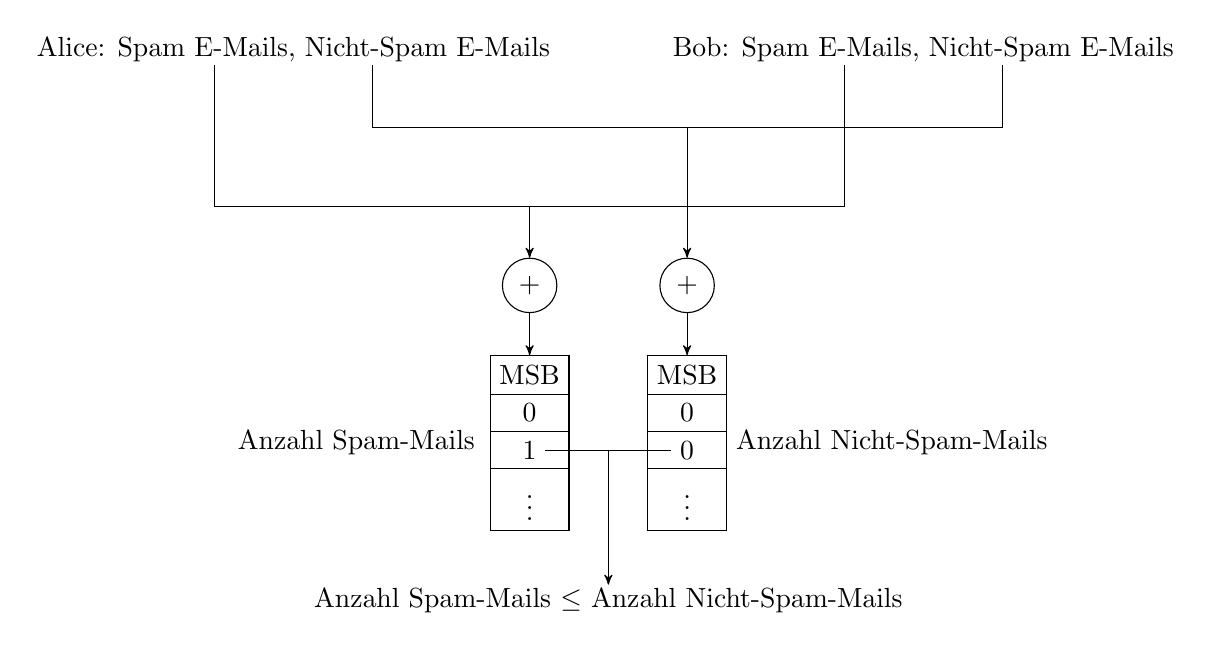
\begin{tikzpicture}
[>=stealth']
\node at (-4, 5) {Alice: Spam E-Mails, Nicht-Spam E-Mails};
\node at (4, 5) {Bob: Spam E-Mails, Nicht-Spam E-Mails};
\node[shape=circle,draw] (spamaddition) at (-1, 2) {+};
\node[shape=circle,draw] (useaddition) at (1, 2) {+};
\node (spamvector) [rectangle split, rectangle split parts=4, draw] at (-1, 0)
{
MSB
\nodepart{second}
0
\nodepart{third}
1
\nodepart{fourth}
\(\vdots\)
};
\node at (-3.2,0) {Anzahl Spam-Mails};

\node(usevector) [rectangle split, rectangle split parts=4, draw] at (1, 0)
{
MSB
\nodepart{second}
0
\nodepart{third}
0
\nodepart{fourth}
\(\vdots\)
};
\node at (3.6,0) {Anzahl Nicht-Spam-Mails};

\draw[->] (spamaddition) to (spamvector);
\draw[->] (useaddition) to (usevector);
\draw (-5, 4.8) -- (-5, 3) -- (3, 3) -- (3, 4.8);
\draw (-3, 4.8) -- (-3, 4) -- (5, 4) -- (5, 4.8);
\draw[->] (-1, 3) to (spamaddition);
\draw[->] (1, 4) to (useaddition);
\draw (-0.8, -0.1) -- (0.8, -0.1);

\draw[->] (0,-0.1) -- (0,-1.8);
\node at (0,-2) {Anzahl Spam-Mails \(\leq\) Anzahl Nicht-Spam-Mails};
\end{tikzpicture}
\caption{High-Level Struktur des Dominierende-Ausgabe-Schaltkreises}
\label{fig:circuit:max sum}
\end{figure}

\subsection{Feststellen ob Ausgabe eindeutig}
\begin{figure}[htb]
\begin{phases}
\aliceknowledge[-2]{Vorwissen};
\aliceknowledge[2]{Eigene diskretisierte E-Mails};

\bobknowledge[-2]{Vorwissen};
\bobknowledge[2]{Eigene diskretisierte E-Mails};

\phase{Phase 4.2: Feststellen ob Ausgabe eindeutig}

\symmetricknowledge{gemeinsamer Blattknoten mit eindeutiger Ausgabe}
\end{phases}
\caption{ID3-Algorithmus, Fall 2: Ausgabe eindeutig}
\end{figure}
Es muss ein Schaltkreis designed werden, der Feststellt, ob alle Elemente
einer Menge eindeutig sind und dann entweder das Klassenlabel oder ein 
Fehlersymbol ausgibt. Die Eingabe ist somit f\"ur jede E-Mail eine
Kodierung f\"ur Spam, Nicht Spam oder Abwesenheit, die Anzahl der Eingaben
ist bekannt und durch die Gesamtanzahl der E-Mails beschr\"ankt.\\
Wir implementieren diesen Schaltkreis dann als Zustandsmaschine, die die
internen Zust\"ande ,,Alles bis hier Spam'', ,,Alles bis hier kein Spam''
und ,,Bereits uneindeutig'' hat. Wenn dann 
\(T \colon \mathrm{State} \times \mathrm{Mailtype}\) ist, muss folgende
Zustands\"ubergangstabelle implementiert werden:\\
\begin{center}
\begin{tabular}{c c c c}
T & Alles bis hier Spam & Alles bis hier kein Spam & Bereits uneindeutig\\
Spam & Alles bis hier Spam & Alles bis hier kein Spam & Bereits Uneindeutig \\
Nicht Spam & Alles bis hier kein Spam & Alles bis hier kein Spam & Bereits Uneindeutig \\
Abwesenheit & Alles bis hier Spam & Alles bis hier kein Spam & Bereits uneindeutig
\end{tabular}
\end{center}
Zudem w\"are es sehr angenehm, wenn die Kodierung von Spam und 
,,Alles bis hier Spam'' und von ,,Nicht Spam'' und ,,Alles bis hier kein Spam''
gleich sind, da dies den Anfangsfall vereinfacht.\\
Wenn wir nun ,,Bereits uneindeutig'' durch 11 kodieren und 
,,Alles bis hier Spam'' mit 01 kodieren und ,,Alles bis hier kein Spam''
mit 00 kodieren und davon ausgehend ,,Spam'' als 01 kodieren und
,,Nicht Spam'' als 00 und ,,Abwesenheit'' als 11, dann muss folgende
Zustands\"ubergangstabelle gelten:\\
\begin{center}
\begin{tabular}{c c c c}
T & 01 & 00 & 11\\
01 & 01 & 11 & 11\\
00 & 11 & 00 & 11\\
11 & 01 & 00 & 11
\end{tabular}
\end{center}

Durch Anwenden von KV-Diagrammen ergeben sich als Zustands\"ubergangsgleichungen
somit, mit \(s_0, s_1\) als Bits des vorherigen Zustandes, \(e_0, e_1\) als Bits
der E-Mail Kodierung und \(s_0', s_1'\) als Bits des neuen Zustandes:
\begin{align*}
s_0' &=& s_0 \vee \overline{s_1} \overline{e_0} e_1
           \vee s_1 \overline{e_0} \overline{e_1}\\
s_1' &=& s_1 \vee s_0 \vee \overline{e_0} e_1
\end{align*}
Der Anfangszustand des Automatens ist die Kodierung der Klasse der ersten E-Mail.
Es muss dann nur noch f\"ur jede E-Mail das beschriebene Zustands\"ubergangsnetz
von den vorherigen Zust\"anden und der Kodierung der Klasse der aktuellen
E-Mail implementiert werden. Das Fehlersymbol, das ausgegeben wird, ist 11,
andernfalls ist die Klasse im zweiten Ausgabebit Kodiert, wobei Spam als 1 
kodiert ist und Nicht Spam als 0.

\subsection{Das Entropien-Protokoll}
\todo[inline]{Schaltkreis f\"ur x * log x -Protokoll aus dem Paper zusammenfassen}

\subsection{Attribut mit maximalem Informationsgewinn finden}
\todo[inline]{Feststellung der benoetigten Bytezahl beschreiben}
\begin{figure}[htb]
\begin{phases}
\aliceknowledge[-2]{Vorwissen};
\aliceknowledge[2]{Eigene diskretisierte E-Mails};

\bobknowledge[-2]{Vorwissen};
\bobknowledge[2]{Eigene diskretisierte E-Mails};

\phase{Phase 4.3: Berechnen der Entropien}

\symmetricknowledge{Gemeinsame Entropien}

\phase{Phase 4.4: Attribut mit maximalem Informationsgewinn finden}

\symmetricknowledge{Gemeinsames bestes aktuelles Attribut}

\phase{Phase 4: Rekursion}

\symmetricknowledge{gemeinsamer Klassifikator}
\end{phases}
\caption{ID3-Algorithmus, Fall 3: Erzeugung eines Astes}
\end{figure}
\todo[inline]{Vorgheen zusammenfassen, Schaltkreis aus dominierender Ausgabe wiederverwenden}

\pagebreak  %XXX: if  possible, kill this pagebreak
\section{Verwenden des Klassifikators}
Es muss zus\"atzlich zum Lern-Programm ein Programm geschrieben
werden, welches den Klassifikator auf eine Menge von E-Mails anwendet.
Wir bieten hierzu ein Programm an, welches den Klassifikator in einem
einfachen Textformat einliest und diesen auf eine Menge von E-Mails
anwendet. Diese Menge von E-Mails ist als Dateien in einem Verzeichnis
gegeben und f\"ur jeden Dateinamen wird eine Klassifikation als Spam
oder Not Spam ausgegeben.
\subsection{Eingabe des Klassifikators}
Ausgehend von den Definitionen eines Attributes und eines Entscheidungsbaumes
kann leicht eine Grammatik erzeugt werden, welche die Form des eingegebenen
Klassifikators eindeutig bestimmt. Wir notieren diese Grammatik in BNF. Diese
ist so gew\"ahlt, dass sie eine LL(1)-Grammatik ist, d.h., sie ist besonders
einfach zu parsen.\\
\begin{verbatim}
tree -> `Decide' `(' attribute (`,' tree)+ `)'
      | `Output' `(' class `)'.
class -> `Spam' | `Not Spam'.
attribute -> `(' word `,' probability `,' probabilty `)'.
word ->   (`a' | `b' | ... | `z' | `A' | ... | `Z')+
probability -> number `.' number .
number -> (`0' | `1' | ... | `9')+.
\end{verbatim}

Somit w\"are ein kodierter Klassifikationsbaum beispielsweise:
\begin{verbatim}
Decide((Foo, 0.3, 0.6),
        Output(Spam), 
        Decide((Bar, 0.5, 0.6), 
                Output(Spam), 
                Output(Not Spam)
              )
      )
\end{verbatim}

Die Produktion ,,probability'' beschreibt eine Zahl, die sich als
eine Folge von Ziffern vor einem Dezimalpunkt und einer Folge von
Ziffern nach dem Dezimalpunkt beschreiben lassen. Dies sind alle
reellen Zahlen, und da wir keine komplexen Zahlen betrachten, sondern
nur Verh\"altnisse von nat\"urlichen Zahlen zueinander ist diese
Darstellung ausreichend, um alle m\"oglichen Zahlenwerte darzustellen.
Da die Buchstabenmenge als die lateinischen Klein- und Grossbuchstaben
definiert ist und ein Wort definiert ist als Sequenz dieser Zeichen,
ist die Produktion ,,word''  ausreichend, um alle m\"oglichen Worte
darzustellen. Damit ergibt sich, dass die Produktion 
,,attribute'' in der Lage ist, alle Attribute, die in dieser
Anwendung auftreten k\"onnen, darzustellen.\\
Es gibt desweiteren bei uns nur die Ausgaben ,,Spam'' und ,,Nicht Spam''.
Damit ist die Produktion ,,class'' ausreichend, um alle 
m\"oglichen Ausgaben des Baumes darzustellen. Daraus folgt, dass die
zweite Produktion von tree in der Lage ist, alle m\"oglichen Bl\"atter
darzustellen. Desweiteren folgt induktiv aus der Vollst\"andigkeit der
Produktion ,,attribute'' und der Darstellbarkeit der Bl\"atter als
Induktionsanfang, dass die erste Produktion von tree in der Lage ist,
alle m\"oglichen auszugebenden Entscheidungsb\"aume darzustellen. Damit
ist die Grammatik m\"achtig genug f\"ur unsere Zwecke.\\
Es ist weiterhin zu bemerken, dass eine semantische Validierung notwendig
ist, da in der Grammatik weder gefordert ist, dass der untere Schwellwert
eines Attributes wirklich kleiner ist als der obere Schwellwert 
eines Attributes noch dass beide Schwellwerte zwischen 0 und 1 liegen, noch
dass die Anzahl der Teilb\"aume richtig ist. Damit ergeben sich die folgenden
Akzeptanzkriterien:\\
\requirement{Der Klassifizierer weist die Eingabe Decide((Foo, 0.5,2),
Output(Spam), Output(Spam)) wegen eines zu grossen Schwellwertes zur\"uck}
\requirement{Der Klassifizierer weist die Eingabe Decide((Foo, 2, 3),
Output(Spam), Output(Spam)) wegen eines zu grossen Schwellwertes zur\"uck}
\requirement{Der Klassifizierer weist die Eingabe Decide((Foo, 1, 0),
Output(Spam), Output(Spam)) wegen falsch sortierter Schwellwerte zur\"uck}
\requirement{Der Klassifizierer weist die Eingabe Decide((Foo, 0.2, 0.3),
Output(Spam), Output(Spam)) wegen zuweniger Teilb\"aume zur\"uck}
\requirement{Der Klassifizierer weist die Eingabe Decide((Foo, 0.2, 0.3),
Output(Spam), Output(Spam), Output(Spam), Output(Spam)) wegen zuvieler
Teilb\"aume zur\"uck}
\requirement{Der Klassifizierer akzeptiert die Eingabe 
Decide((Foo, 0.2, 0.3), 
    Output(Spam),
    Decide((Bar, 0.3, 0.4)
        Output(Spam),
        Output(Not Spam), 
        Output(Spam)),
    Output(Spam))}
\requirement{Der Klassifizierer akzeptiert die Eingabe Decide((Foo, 0, 0.5),
Output(Spam), Output(Spam))}
\requirement{Der Klassifizierer akzeptiert die Eingabe Decide((Foo, 0.5, 1),
Output(Spam), Output(Spam))}
\requirement{Der Klassifizierer akzeptiert die Eingabe 
Decide((Foo, 0.5, 0.5)), Output(Spam), Output(Spam))}
\requirement{Der Klassifizierer akzeptiert die Eingabe Decide((Foo, 0, 0),
Output(Spam))}
\requirement{Der Klassifizierer akzeptiert die Eingabe Decide((Foo, 1, 1),
Output(Spam))}
\subsection{Arbeitsweise des Klassifikators}
Der Klassifikator bekommt als Eingabe ein Verzeichnis mit E-Mails und eine
Datei meinem einem Klassifikator. Den Klassifikator liest er ein und
speichert ihn intern. Danach traversiert der Klassifikator das gegebene
Verzeichnis rekursiv und behandelt jede Datei, die er in diesem Verzeichnis
findet als E-Mail-Inhalt. (Dadurch ist es m\"oglich, die Trainingsdaten auch
als Versuchsdaten zu benutzen, ohne sie zu bewegen).\\
F\"ur jede E-Mail wird dann der Inhalt der E-Mail eingelesen und die
Klassifikation durch den eingegebenen Klassifikator durchgef\"uhrt, d.h., 
f\"ur jeden Ast werden die Vorkommnisse des Wortes im Attribut
festgestellt und rekursiv im entsprechenden Teilbaum weiterklassifiziert
und in einem Blatt wird die Klasse festgestellt. Diese festgestellte Klasse
wird dann zusammen mit dem relativen Pfad vom eingegebenen Verzeichnis
ausgegeben.\\
Wenn also beispielsweise folgende Verzeichnisstruktur gegeben ist:
\begin{verbatim}
mails/hank/mail1
mails/hank/mail2
mails/bob/mail1
\end{verbatim}
und wir annehmen, dass der eingegebene Klassifikator E-Mails mit dem Index
1 als Spam erkennt und E-Mails mit dem Index 2 als Nicht Spam, dann
w\"are die Ausgabe:
\begin{verbatim}
hank/mail1 Spam
hank/mail2 Not Spam
bob/mail1 Spam
\end{verbatim}
Damit ergeben sich folgende Akzeptanzkriterien:\\
\requirement{Gegeben der Klassifikator Decision((Bar, 0.3, 0.6), Output(Spam),
Output(Not Spam), Output(Spam)), dann wird die E-Mail "Bar Foo Foo Foo" als
Spam klassifiziert}
\requirement{Gegeben der Klassifikator Decision((Bar, 0.3, 0.6), Output(Spam),
Output(Not Spam), Output(Spam)), dann wird die E-Mail "Bar, Bar, Foo, Foo" als
Not Spam klassifiziert}
\requirement{Gegeben der Klassifikator Decision((Bar, 0.3, 0.6), Output(Spam),
Output(Not Spam), Output(Spam)), dann wird die E-Mail "Bar, Bar, Bar, Foo" als
Spam klassifiziert}
\requirement{Gegen der Klassifikator Decision((Bar, 0.3, 0.6), Output(Spam),
Output(Not Spam), Output(Spam)) und eine Verzeichnisstruktur wie oben
skizziert, wobei hank/mail1 "Bar Foo Foo Foo", hank/mail2 "Bar Bar Foo Foo"
und bob/mail1 "Bar Bar Bar Foo" enth\"alt, dann wird die oben als Beispiel
genannte Ausgabe produziert (oder in einer anderen Reihenfolge}
\end{document}
